\documentclass{beamer}
\usepackage[utf8]{inputenc}
\usepackage{tabularx}
\usepackage{mathrsfs}
\usepackage{pgf}
\usepackage{amsmath}
\usepackage{array}
\usepackage{pifont}% http://ctan.org/pkg/pifont
\newcommand{\cmark}{\ding{51}}%
\newcommand{\xmark}{\ding{55}}%
% \usepackage{enumitem}
\usepackage[ruled]{algorithm2e}
\usepackage{underoverlap}

% \usepackage{algorithm}
\usepackage{algpseudocode}

\usepackage{tikz}
\usetikzlibrary{calc, chains, decorations.pathmorphing}
\usetikzlibrary{shapes.geometric}
\usetikzlibrary{arrows,shapes,positioning}
\usetikzlibrary{calc,decorations.markings}
\usetikzlibrary{decorations.text}
\usetikzlibrary{patterns}
\usetikzlibrary{arrows.meta}
\usepackage{color, soul}


\definecolor{top-darkblue}{RGB}{62,78,99} 
\definecolor{foot-darkblue}{RGB}{77,82,151} 
\definecolor{foot-blue}{RGB}{171,200,230} 
\definecolor{title-blue}{RGB}{0,76,153}

\definecolor{block-red}{rgb}{1.1, 0.41, 0.38}
\definecolor{propa-grey}{rgb}{0.82, 0.84, 0.86}
\definecolor{true-green}{RGB}{182,191,0}%{rgb}{0, 0.8, 0.2}
\definecolor{purple}{rgb}{0.74, 0.2, 0.64}
\definecolor{cons-red}{rgb}{0.5, 0.11, 0.11}

\definecolor{UPMCEngagementBlueA} {RGB}{140,184,198}
\definecolor{UPMCEngagementBlueB} {RGB}{92,127,146}

\definecolor{UPMCCorporateGreen} {RGB}{182,191,0}
\definecolor{UPMCExcellenceOrangeA} {RGB}{224,82,6}
\definecolor{UPMCExcellenceOrangeB} {RGB}{225,160,47}

\mode<presentation> {
  \usetheme[not@ku={UPMC}, wide, TPomitframeno, FTalign=left,%
  greyfoot, fnolabel=, basecolour=UPMCEngagementBlueB,%
  sidebar=0pt]{Frederiksberg}
  \setbeamercolor{block title example}{bg=UPMCCorporateGreen}
  \setbeamercolor{block title alerted}{bg=UPMCExcellenceOrangeA}
  \setbeamercolor{alerted text}{fg=UPMCExcellenceOrangeA}
  \setbeamertemplate{headline}{}
  \setbeamertemplate{footline}[page number]{}
  \setbeamercovered{transparent}
  \beamertemplatenavigationsymbolsempty
}

\definecolor{red}{rgb}{0.7, 0.11, 0.11}
\definecolor{green}{rgb}{0, 0.8, 0.2}

\tikzstyle{point}=[circle,draw,thick,fill=black,scale=0.2]
\tikzstyle{point+}=[circle,draw=red,thick,fill=red,scale=0.3]
\tikzstyle{class2}=[ellipse, draw, minimum width=2cm, minimum height=1cm]
\tikzstyle{class1}=[ellipse, draw, minimum width=1cm, minimum height=1cm]

\tikzstyle{decision}=[circle,draw,thick,fill=UPMCEngagementBlueA]
\tikzstyle{decision-graph}=[text width={width("$\neg x_3@3$")},circle,
align=center,draw,thick,fill=yellow]
\tikzstyle{propa-graph}=[text width={width("$\neg x_3@3$")},circle,draw,thick,
align=center,fill=propa-grey]
\tikzstyle{conflict}=[<->,>=latex,rounded corners=5pt,thick,draw=blue, line width=1mm]
\tikzstyle{uip}=[draw=true-green,ultra thick]
\tikzstyle{cut}=[-,>=stealth,rounded corners=5pt,thick,draw=blue, line width=0.4mm]
\tikzstyle{link}=[->,>=latex,rounded corners=5pt,thick]
\tikzstyle{unsat}=[draw,thick,fill=red]
\tikzstyle{sat}=[draw,thick,fill=green]
\tikzstyle{propa}=[draw,thick,fill=propa-grey]
\tikzstyle{backtrack}=[->,>=latex,dashed,rounded corners=20pt,thick,draw=blue, line width=0.5mm]

\setbeamertemplate{footline}[frame number]{}

% Definition of variable
\def\SAT{\textcolor{green}{\texttt{SAT}}}
\def\UNSAT{\textcolor{red}{\texttt{UNSAT}}}

\def\true{\textcolor{green}{\texttt{true}}}
\def\false{\textcolor{red}{\texttt{false}}}

\def\ok{\textcolor{green}{\cmark}}
\def\ko{\textcolor{red}{\xmark}}



\tikzset{onslide/.code args={<#1>#2}{%
		\only<#1>{\pgfkeysalso{#2}} % \pgfkeysalso doesn't change the path
}}

\definecolor{hgreen}{RGB}{0,153,20}%{rgb}{0, 0.8, 0.2}
\newcommand{\cred}[1]{{\color{red}#1}}
\newcommand{\cgreen}[1]{{\color{hgreen}#1}}
\newcommand{\cblue}[1]{{\color{blue!80}#1}}
\newcommand{\cprop}[1]{{\color{orange}#1}}



\begin{document}

\author{Hakan \textsc{METIN}}

\begin{frame}
\frametitle{Exploitation des symétries dynamiques pour la résolution des problèmes SAT}
\framesubtitle{Thèse de doctorat de Sorbonne Université}
 
   Hakan \textsc{Metin}\\
  \vfill
  %\begin{center}

	\scriptsize
    \begin{tabular}{ll}
  	    \textbf{Supervisors:} & \\
    	\textsc{Souheib Baarir}  & Maître de conférences, Université Paris Nanterre\\
    	\vspace{1em}
    	\textsc{Fabrice Kordon}  & Professeur, Sorbonne Université\\
 	    \textbf{Jury Members:} & \\
    	\textsc{Pascal \textsc{Fontaine}}  &  Maître de conférences, Université de Lorraine\\
    	\textsc{Laure Petrucci}  & Professeur, Université Paris 13\\
    	\textsc{Jean-Michel	Couvreur}  & Professeur, Université d'Orléans\\
    	\textsc{Emanuelle Encrenaz}  & Maître de conférences, Sorbonne Université\\
    	\textsc{Souheib Baarir}  & Maître de conférences, Université Paris Nanterre\\
    	\textsc{Fabrice Kordon}  & Professeur, Sorbonne Université\\
    \end{tabular}\\
 % \end{center}

  \vskip 3ex
  \begin{columns}[t]
    \begin{column}[T]{\textwidth}
      \includegraphics[height=1.2cm]{images/logo_sorbonne}
      \hfill
      \includegraphics[height=1.3cm]{images/lip6}
      \centering
    \end{column}
  \end{columns}
\end{frame}

%% ----------------------------------------------------------------------------
\begin{frame}

\frametitle{Motivation}
	\begin{itemize}
		\item planning
		\item scheduling
		\item combinatorial design
		\item system analysis (model-checking)
		\item etc
	\end{itemize}
\end{frame}
%% ----------------------------------------------------------------------------

\begin{frame}

\tikzstyle{every picture}+=[remember picture]
\frametitle{SAT an example}
\everymath{\displaystyle}
\centering


\begin{tabular}{ccc}
	\includegraphics[scale=0.07]{images/room} & \includegraphics[scale=0.07]{images/room}& \includegraphics[scale=0.07]{images/room}\\
	\tikz[baseline]{\node[anchor=base] (t1){1};} & \tikz[baseline]{\node[anchor=base] (t2){2};} & \tikz[baseline]{\node[anchor=base] (t3){3};}\\
	 & & \\
	\tikz[baseline]{\node[anchor=base] (s1){};} & \tikz[baseline]{\node[anchor=base] (s2){};} & \tikz[baseline]{\node[anchor=base] (s3){};}\\
	
\includegraphics[scale=0.1]{images/south} & 
\includegraphics[scale=0.1]{images/simpson} & 
\includegraphics[scale=0.09]{images/titeuf}\\
	A                                        & B                                           & C\\
\end{tabular}

\begin{tikzpicture}[overlay]
\tikzstyle{line} = [<-, line width=0.5mm];
\path[line]<1> (t1) edge  (s1.south);
\path[line]<1> (t2) edge  (s2.south);
\path[line]<1> (t3) edge  (s3.south);

\path[line]<2> (t1) edge  (s2.south);
\path[line]<2> (t2) edge  (s1.south);
\path[line]<2> (t3) edge  (s3.south);

\path[line]<3> (t1) edge  (s1.south);
\path[line]<3> (t2) edge  (s3.south);
\path[line]<3> (t3) edge  (s2.south);

\path[line]<4> (t2) edge  (s1.south);
\path[line]<4> (t3) edge  (s2.south);
\path[line]<4> (t1) edge  (s3.south);

\path[line]<5> (t1) edge  (s2.south);
\path[line]<5> (t2) edge  (s3.south);
\path[line]<5> (t3) edge  (s1.south);

\end{tikzpicture}

\vfill
Attribute each group to a class room
\end{frame}
%% ----------------------------------------------------------------------------

\begin{frame}

\tikzstyle{every picture}+=[remember picture]
\frametitle{SAT an example 2 }
\everymath{\displaystyle}
\centering

\begin{tabular}{cc}
	\includegraphics[scale=0.07]{images/room} & \includegraphics[scale=0.07]{images/room}\\
	\tikz[baseline]{\node[anchor=base] (r1){1};} & \tikz[baseline]{\node[anchor=base] (r2){2};}\\
\end{tabular}

\begin{tabular}{ccc}
	\tikz[baseline]{\node[anchor=base] (g1){};} & \tikz[baseline]{\node[anchor=base] (g2){};} & \tikz[baseline]{\node[anchor=base] (g3){};}\\
	
\includegraphics[scale=0.1]{images/south} & 
\includegraphics[scale=0.1]{images/simpson} & 
\includegraphics[scale=0.09]{images/titeuf}\\
	A                                        & B                                           & C\\
\end{tabular}

\begin{tikzpicture}[overlay]
\tikzstyle{line} = [<-, line width=0.5mm];
\path[line]<2> (r1) edge  (g1.south);
\path[line]<2> (r2) edge  (g2.south);

\path[line]<3> (r1) edge  (g2.south);
\path[line]<3> (r2) edge  (g1.south);

\path[line]<4> (r1) edge  (g1.south);
\path[line]<4> (r2) edge  (g3.south);

\path[line]<5> (r1) edge  (g3.south);
\path[line]<5> (r2) edge  (g1.south);


\path[line]<6> (r1) edge  (g2.south);
\path[line]<6> (r2) edge  (g3.south);

\path[line]<7> (r1) edge  (g3.south);
\path[line]<7> (r2) edge  (g2.south);

\end{tikzpicture}

\vfill
Attribute each group to a class room
\end{frame}

%\begin{frame}
%  \frametitle{SAT an example}
%  
%  \centering
% \begin{tabular}{c|c |c}
% 	  \includegraphics[scale=0.07]{images/room} & \includegraphics[scale=0.07]{images/room}& \includegraphics[scale=0.07]{images/room}\\
% 	   1                                        & 2                                        & 3\\
% \end{tabular}
%\vfill
% \begin{tabular}{c|c|c}
%	
\includegraphics[scale=0.1]{images/south} & 
\includegraphics[scale=0.1]{images/simpson} & 
\includegraphics[scale=0.09]{images/titeuf}\\
%	 A                                        & B                                           & C\\
%\end{tabular}
%\vfill
%Attribute each group to a class room
%\end{frame}
%% ----------------------------------------------------------------------------
\begin{frame}
\frametitle{Encoding the problem}
\begin{columns}
	\begin{column}{0.1\textwidth}
		\small
	$(A,1) (A,2) (A,3)$\\
	$(B,1) (B,2) (B,3)$\\
	$(C,1) (C,2) (C,3)$\\
	\vspace{1em}
	$ \neg (A,1)  \neg (B,1)$\\
	$ \neg (A,1)  \neg (C,1)$\\
	$ \neg (B,1)  \neg (C,1)$\\
	\vspace{1em}
	$ \neg (A,2)  \neg (B,2)$\\
	$ \neg (A,2)  \neg (C,2)$\\
	$ \neg (B,2)  \neg (C,2)$\\
	\vspace{1em}
	$ \neg (A,3)  \neg (B,3)$\\
	$ \neg (A,3)  \neg (C,3)$\\
	$ \neg (B,3)  \neg (C,3)$\\
	\end{column}
	\begin{column}{0.2\textwidth}  %%<--- here
		\small
$ x_1 \lor  x_2 \lor x_3 $ \\
$x_4 \lor  x_5 \lor x_6 $ \\
$x_7 \lor  x_8 \lor x_9 $ \\
	\vspace{1em}
$ \neg x_1 \lor  \neg x_4 $ \\
$ \neg x_1 \lor  \neg x_7 $ \\
$ \neg x_4 \lor  \neg x_7 $ \\
	\vspace{1em}
$\neg x_2 \lor  \neg x_5 $ \\
$ \neg x_2 \lor  \neg x_8 $ \\
$ \neg x_5 \lor  \neg x_8 $ \\
	\vspace{1em}
$ \neg x_3 \lor  \neg x_6 $ \\
$ \neg x_3 \lor  \neg x_9 $ \\
$ \neg x_6 \lor  \neg x_9 $ \\
	\end{column}
\end{columns}

%$\omega_1 = x_1 \lor  x_2 \lor x_3 $ \\
%$\omega_2 = x_4 \lor  x_5 \lor x_6 $ \\
%$\omega_3 = x_7 \lor  x_8 \lor x_9 $ \\
%\vspace{1em}
%$\omega_4 = \neg x_1 \lor  \neg x_4 $ \\
%$\omega_5 = \neg x_1 \lor  \neg x_7 $ \\
%$\omega_6 = \neg x_4 \lor  \neg x_7 $ \\
%\vspace{1em}
%$\omega_7 = \neg x_2 \lor  \neg x_5 $ \\
%$\omega_8 = \neg x_2 \lor  \neg x_8 $ \\
%$\omega_9 = \neg x_5 \lor  \neg x_8 $ \\
%\vspace{1em}
%$\omega_{10} = \neg x_3 \lor  \neg x_6 $ \\
%$\omega_{11} = \neg x_3 \lor  \neg x_9 $ \\
%$\omega_{12} = \neg x_6 \lor  \neg x_9 $ \\

\end{frame}

%% ----------------------------------------------------------------------------
\begin{frame}
\frametitle{Encoding the problem}
\begin{columns}
	\begin{column}{0.1\textwidth}
		\small
		$(A,1) (A,2) $\\
		$(B,1) (B,2) $\\
		$(C,1) (C,2) $\\
		\vspace{1em}
		$ \neg (A,1)  \neg (B,1)$\\
		$ \neg (A,1)  \neg (C,1)$\\
		$ \neg (B,1)  \neg (C,1)$\\
		\vspace{1em}
		$ \neg (A,2)  \neg (B,2)$\\
		$ \neg (A,2)  \neg (C,2)$\\
		$ \neg (B,2)  \neg (C,2)$\\
	\end{column}
	\begin{column}{0.2\textwidth}  %%<--- here
		\small
		$ x_1 \lor  x_2 $ \\
		$x_3 \lor  x_4  $ \\
		$x_5 \lor  x_6 $ \\
		\vspace{1em}
		$ \neg x_1 \lor  \neg x_3 $ \\
		$ \neg x_1 \lor  \neg x_5 $ \\
		$ \neg x_3 \lor  \neg x_5 $ \\
		\vspace{1em}
		$\neg x_2 \lor  \neg x_4 $ \\
		$ \neg x_2 \lor  \neg x_6 $ \\
		$ \neg x_4 \lor  \neg x_6 $ \\
	\end{column}
\end{columns}

%$\omega_1 = x_1 \lor  x_2 \lor x_3 $ \\
%$\omega_2 = x_4 \lor  x_5 \lor x_6 $ \\
%$\omega_3 = x_7 \lor  x_8 \lor x_9 $ \\
%\vspace{1em}
%$\omega_4 = \neg x_1 \lor  \neg x_4 $ \\
%$\omega_5 = \neg x_1 \lor  \neg x_7 $ \\
%$\omega_6 = \neg x_4 \lor  \neg x_7 $ \\
%\vspace{1em}
%$\omega_7 = \neg x_2 \lor  \neg x_5 $ \\
%$\omega_8 = \neg x_2 \lor  \neg x_8 $ \\
%$\omega_9 = \neg x_5 \lor  \neg x_8 $ \\
%\vspace{1em}
%$\omega_{10} = \neg x_3 \lor  \neg x_6 $ \\
%$\omega_{11} = \neg x_3 \lor  \neg x_9 $ \\
%$\omega_{12} = \neg x_6 \lor  \neg x_9 $ \\

\end{frame}
%% ----------------------------------------------------------------------------
\begin{frame}
\frametitle{SAT}
\centering
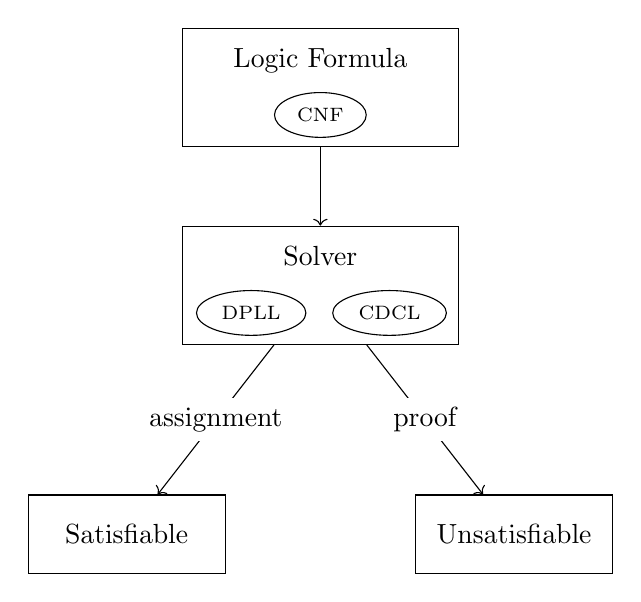
\begin{tikzpicture}
\tikzstyle{box} = [draw, minimum height = 1.5cm, minimum width=3.5cm,
				anchor=north,text centered,text width = 0.25\textwidth, text depth = .75cm]
\tikzstyle{result} = [draw, minimum width=2.5cm, minimum height=1cm]
\node[box] (input) {Logic Formula};    

\node<2->[draw, ellipse] (cnf) at ($(input) + (0pt, -10pt)$) {\scriptsize CNF};

\node[box] (solver) at ($(input) + (0pt, -50pt)$) {Solver};
\node<3->[draw, ellipse] (cnf) at ($(solver) + (-25pt, -10pt)$) {\scriptsize DPLL};
\node<3->[draw, ellipse] (cnf) at ($(solver) + (25pt, -10pt)$) {\scriptsize CDCL};

\node[result] (sat) at ($(solver) + (-70pt, -90pt)$) {Satisfiable};
\node[result] (unsat) at ($(solver) + (70pt, -90pt)$) {Unsatisfiable};

\draw[->] (input) -> (solver);
\draw[->] (solver) -> node[midway,fill=white] {assignment}  (sat);
\draw[->] (solver) -> node[midway,fill=white] {proof}(unsat);
\end{tikzpicture}

\end{frame}


%% ----------------------------------------------------------------------------
\begin{frame}
\frametitle{Conjunctive Normal Form (CNF)}
\scriptsize

$(x_2 x_3)(x_5 x_6)(x_8 x_9)(\neg x_2 \neg x_3)(\neg x_5 \neg x_6)(\neg x_8 \neg x_9)$
$(x_4 x_7)(x_5 x_8)(x_6 x_9)(\neg x_4 \neg x_7)(\neg x_5 \neg x_8)(\neg x_6 \neg x_9)$\\
$(x_1 x_2)(x_4 x_5)(x_7 x_8)(\neg x_1 \neg x_2)(\neg x_4 \neg x_5)(\neg x_7 \neg x_8)$\\
$(x_1 x_4)(x_2 x_5)(x_3 x_6)(\neg x_1 \neg x_4)(\neg x_2 \neg x_5)(\neg x_3 \neg x_6)$\\
	
	
	$(x_2 x_3)(x_5 x_6)(x_8 x_9)$\\
	$(x_4 x_7)(x_5 x_8)(x_6 x_9)$\\
	$(x_1 x_2)(x_4 x_5)(x_7 x_8)$\\
	$(x_1 x_4)(x_2 x_5)(x_3 x_6)$\\
	
	\vfill
	

$
(x_1 \lor x_2 \lor x_3) \land
(x_4 \lor x_5 \lor x_6) \land
(x_7 \lor x_8 \lor x_9) \land
(\neg x_1 \lor \neg x_4) \land
(\neg x_1 \lor \neg x_7) \land
(\neg x_4 \lor \neg x_7) \land
(\neg x_2 \lor \neg x_5) \land
(\neg x_2 \lor \neg x_8) \land
(\neg x_5 \lor \neg x_8) \land
(\neg x_3 \lor \neg x_6) \land
(\neg x_3 \lor \neg x_9) \land
(\neg x_6 \lor \neg x_9) 
$
\end{frame}


\begin{frame}
  \frametitle{Computing symmetries of a SAT problem}
% \setlength{\tabcolsep}{35pt}

\newcolumntype{C}{ >{\centering\arraybackslash} m{5cm} }
\newcolumntype{D}{ >{\centering\arraybackslash} m{1cm} }
\begin{tabular}{CC}
	$CNF\ formula$ &{\scriptsize
		\begin{tabular}{c}
			$(x_1 \lor x_2 \lor x_3) \land
			(x_4 \lor x_5 \lor x_6) \land
			(x_7 \lor x_8 \lor x_9) $\\
			$\land (\neg x_1 \lor \neg x_4) \land
			(\neg x_1 \lor \neg x_7) \land
			(\neg x_4 \lor \neg x_7)$\\
			$\land (\neg x_2 \lor \neg x_5) \land
			(\neg x_2 \lor \neg x_8) \land
			(\neg x_5 \lor \neg x_8)$ \\
			$\land (\neg x_3 \lor \neg x_6) \land
			(\neg x_3 \lor \neg x_9) \land
			(\neg x_6 \lor \neg x_9)$\\
	\end{tabular}}\\
	\visible<2-> {
		
		$\Downarrow$ & $\Downarrow$  \\
		
		colored graph & 
		\includegraphics[scale=0.27]{example-image-a}\\ \\
	}
	\visible<3-> {
		$\|$ & $\|$  \\
		
		graph automorphism & 
		\small{(\texttt{bliss} \footnote{http://www.tcs.hut.fi/Software/bliss/} or 
			\texttt{saucy} \footnote{http://vlsicad.eecs.umich.edu/BK/SAUCY/})} 
		\\
	}
	\visible<4-> {
		$\Downarrow$ & $\Downarrow$  \\
		
		set of symmetries & 
					\scriptsize
		\begin{tabular}{c}
			$g_1 = (x_2 \enspace x_3)(x_5 \enspace x_6)(x_8 \enspace x_9)$\\
			$g_2 = (x_4 \enspace x_7)(x_5 \enspace x_8)(x_6 \enspace x_9)$\\
			$g_3 = (x_1 \enspace x_2)(x_4 \enspace x_5)(x_7 \enspace x_8)$\\
			$g_4 = (x_1 \enspace x_4)(x_2 \enspace x_5)(x_3 \enspace x_6)$
		\end{tabular}
	}
\end{tabular}
\end{frame}
%% ----------------------------------------------------------------------------
\begin{frame}
\frametitle{SAT}
%	Algorithm solving 
%	CDCL
%	
%	NP complete problem

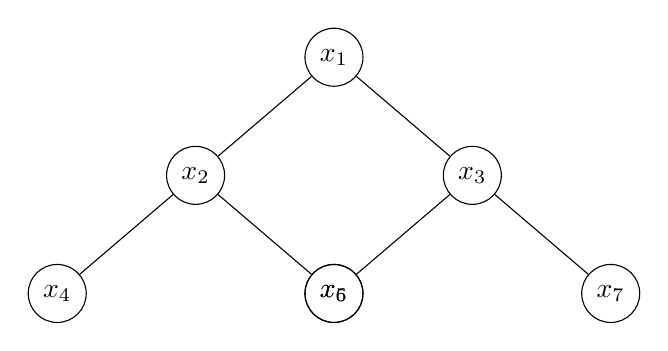
\begin{tikzpicture}[sibling distance=10em,]
\tikzstyle{e} = [draw, circle];
	\node[e](top) {$x_1$}
		child % level 1 left
		{
			 node[e](l) {$x_2$}
			 child { % level 2.1 left
			 	node[e](ll) {$x_4$}
			 }
		 	child { % level 2.1 right
		 		node[e](lr){$x_5$}
		 	}
		}
		child { % level 1 right
			 node[e](r) {$x_3$}
			  child { % level 2.2 left
			 	node[e](rl) {$x_6$}
			 }
			 child { % level 2.2 right
			 	node[e](rr){$x_7	$}
			 }
		};
	
\end{tikzpicture}


\end{frame}
%% ----------------------------------------------------------------------------
\begin{frame}
\frametitle{SAT}
	example solving arbre
	
\end{frame}
%% ----------------------------------------------------------------------------
\begin{frame}
\frametitle{Conflict Driven Clause Learning Algorithm (CDCL)}

\centering

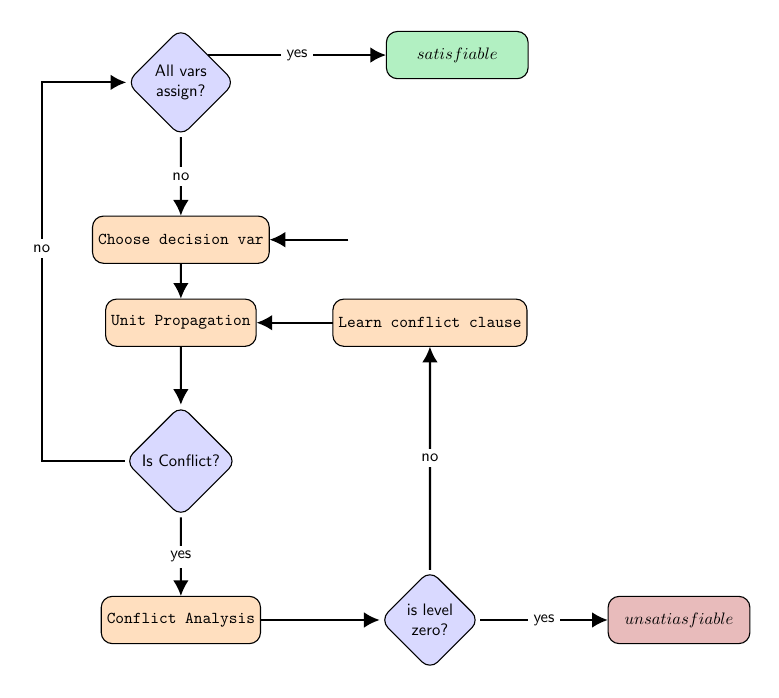
\begin{tikzpicture}[scale=1,every node/.style={scale=0.6,fill=white, font=\sffamily}, align=center]
	% Specification of nodes (position, etc.)
	\tikzset{%	
		>={Latex[width=2mm,length=2mm]},
		% Specifications for style of nodes:
		base/.style = {rectangle, rounded corners, draw=black,
			minimum width=2cm, minimum height=1cm,
			text centered, font=\sffamily},
		question/.style = {base, diamond, fill=blue!15},
		question/.style = {base, diamond, fill=blue!15},
		unsat/.style = {base, fill=red!30,minimum width=3cm},
		sat/.style = {base, fill=green!30,minimum width=3cm},
		process/.style = {base, minimum width=2.5cm, fill=orange!25,
			font=\ttfamily},
		processcurr/.style = {process, thick, line width=0.7mm, draw=purple!80 },
		questioncurr/.style = {question,line width=0.7mm, draw=purple!80},
		line/.style = {->, thick },
		linecurr/.style = {line, line width=0.7mm, draw=purple!80},
	}
	\node (isfin) [question] {All vars\\ assign?};
	\node (dec)     [process, below = of isfin]          {Choose decision var};
	\node (sdec)     [right = of dec]          {};
	\node (idec) [left = of isfin]  {};
	\node (prop)    [process] at ($(dec) + (0pt, -30pt)$)          {Unit Propagation};
	\node (conf)    [question] at ($(prop) + (0pt, -50pt)$){ Is Conflict?};
	\node (confanalyse) [process, below = of conf] {Conflict Analysis};
	\node (learn) [process] at ($(prop) + (90pt, 0)$) {Learn conflict clause};
	\node (isend) [question] at ($(confanalyse) + (90pt, 0)$) {is level\\zero?};
	\node (end) [unsat] at ($(isend) + (90pt, 0)$) {$unsatiasfiable$};
	\node (ends) [sat] at ($(isfin.north east) + (+90pt, 0)$){$satisfiable$};
	
	\draw[line]     (sdec) -- (dec);
	\draw[line]     (dec) -- (prop);
	\draw[line]     (prop) -- (conf);
	\draw[line]     (conf) -| node [yshift=4.5 cm] {no}(idec.center) -- (isfin);
	\draw[line]     (conf) -- node {yes} (confanalyse);
	\draw[line]     (isfin) -- node {no}(dec);
	\draw[line]     (confanalyse) --(isend);
	\draw[line]     (isend) -- node {yes}(end);
	\draw[line]     (isfin.north east) -- node {yes}(ends);
	\draw[line]     (learn) -- (prop);
	\draw[line]     (isend) -- node [] {no}(learn);	
	\end{tikzpicture}

\end{frame}
%% ----------------------------------------------------------------------------
\begin{frame}
\frametitle{TEST Conflict Driven Clause Learning Algorithm (CDCL)}

\centering

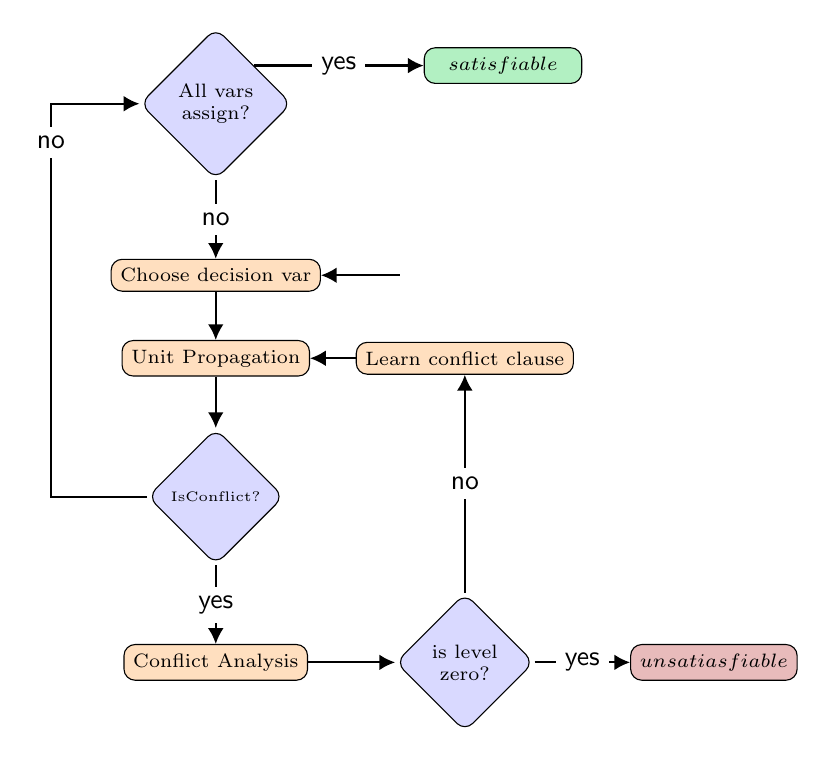
\begin{tikzpicture}[scale=1,every node/.style={scale=1,fill=white, font=\sffamily}, align=center]
% Specification of nodes (position, etc.)
%    \tikzstyle{every node}=[font=\small]
\tikzset{%	
	>={Latex[width=2mm,length=2mm]},
	% Specifications for style of nodes:
	base/.style = {rectangle, rounded corners, draw=black,
		text centered, font=\scriptsize},
	question/.style = {draw, diamond, fill=blue!15, font=\tiny},
	question/.style = {base, diamond, fill=blue!15},
	unsat/.style = {base, fill=red!30,minimum width=2cm},
	sat/.style = {base, fill=green!30,minimum width=2cm},
	process/.style = {base, fill=orange!25,
		font=\scriptsize},
	processcurr/.style = {process, thick, line width=0.7mm, draw=purple!80 },
	questioncurr/.style = {question,line width=0.7mm, draw=purple!80},
	line/.style = {->, thick },
	linecurr/.style = {line, line width=0.7mm, draw=purple!80},
}
\node (isfin) [question] { All vars\\ assign?};
\node (dec)     [process, below = of isfin]          {Choose decision var};
\node (sdec)     [right = of dec]          {};
\node (idec) [left = of isfin]  {};
\node (prop)    [process] at ($(dec) + (0pt, -30pt)$)          {Unit Propagation};
\node (conf)    [question] at ($(prop) + (0pt, -50pt)$){\tiny IsConflict?};
\node (confanalyse) [process, below = of conf] {Conflict Analysis};
\node (learn) [process] at ($(prop) + (90pt, 0)$) {Learn conflict clause};
\node (isend) [question] at ($(confanalyse) + (90pt, 0)$) {is level\\zero?};
\node (end) [unsat] at ($(isend) + (90pt, 0)$) {$unsatiasfiable$};
\node (ends) [sat] at ($(isfin.north east) + (+90pt, 0)$){$satisfiable$};

\draw[line]     (sdec) -- (dec);
\draw[line]     (dec) -- (prop);
\draw[line]     (prop) -- (conf);
\draw[line]     (conf) -| node [yshift=4.5 cm] {no}(idec.center) -- (isfin);
\draw[line]     (conf) -- node {yes} (confanalyse);
\draw[line]     (isfin) -- node {no}(dec);
\draw[line]     (confanalyse) --(isend);
\draw[line]     (isend) -- node {yes}(end);
\draw[line]     (isfin.north east) -- node {yes}(ends);
\draw[line]     (learn) -- (prop);
\draw[line]     (isend) -- node [] {no}(learn);	
\end{tikzpicture}

\end{frame}

%% ----------------------------------------------------------------------------
\begin{frame}
\frametitle{Tree}

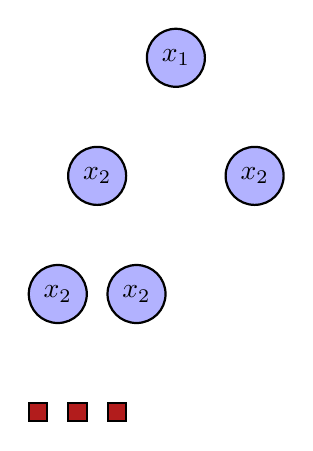
\begin{tikzpicture}
%\def\layersep{1.5cm}
%\def\unitsep{1.5cm}
%
%\foreach \x in {1,...,4}
%\path   node[decision] (L_2_\x) at (\x*\unitsep,2*\layersep){};
%\foreach \x in {1,...,2}
%
%\path   node[decision] (L_3_\x) at ({(1+\x)*\unitsep},3*\layersep){};
%\foreach \x in {1,...,1}
%\path   node[decision] (L_4_\x) at ({(1+\x)*\unitsep},4*\layersep){};


\newcommand{\x}{1}
\newcommand{\y}{-1.5}

\tikzstyle{decision}=[circle,draw,thick,fill=blue!30]
\tikzstyle{unsat}=[draw,thick,fill=red]

    \node[decision](r) at (0,0) {$x_1$};
    \node[decision](l) at (-\x,\y) {$x_2$};
    \node[decision](r) at (\x,\y) {$x_2$};
    
    \node[decision](l) at (-\x-\x*0.5,2*\y) {$x_2$};
    \node[decision](l) at (-\x+\x*0.5,2*\y) {$x_2$};
    
    \node[unsat](l) at (-\x-\x*0.5-\x*0.25,3*\y) {};
    \node[unsat](l) at (-\x-\x*0.5+\x*0.25,3*\y) {};
    
    \node[unsat](l) at (-\x+\x*0.5-\x*0.25,3*\y) {};
    
    
      %\node[unsat](l) at (-\x-\x*0.5+\x*0.25,3*\y) {};
    
%	\node[decision](l) at (-\x,\y) {$x_2$};
%	\node[decision](r) at (\x,\y) {$x_2$};
%	
%	\node[decision](ll) at (-\x*2+\x*0.5*1,2*\y-0.75) {$x_3$};
%	\node[decision](lr) at (-\x*2+\x*0.5*3,2*\y-0.75) {$x_3$};
%	\node[decision](rl) at (-\x*2+\x*0.5*5,2*\y-0.75) {$x_3$};
%	\node[decision](rr) at (-\x*2+\x*0.5*7,2*\y-0.75) {$x_3$};
%	
%	
%	\foreach \x in {0,...,7}
%	\node[unsat](llr) at (-2.75+0.75*\x,-4.5) {};
	
%	\node[decision](x3) at (\x*2-0.75,2*\y-0.5) {$x_5$};
	
\end{tikzpicture}

\end{frame}

%% ----------------------------------------------------------------------------

\begin{frame}[allowframebreaks,noframenumbering]
  \scriptsize
  \nocite{*}
  \bibliographystyle{alpha}
  \bibliography{main}
\end{frame}


\end{document}